\documentclass[11pt]{article}

\usepackage[margin=1in]{geometry}
\usepackage{setspace}
\usepackage{amsmath}
\usepackage{hyperref}
\usepackage{fancyhdr}

% TikZ for system diagram
\usepackage{tikz}
\usetikzlibrary{arrows.meta,positioning,shapes.geometric,fit,calc}

% Header and Footer Configuration
\pagestyle{fancy}

\fancyhf{}

% Header
\fancyhead[L]{CSI 4150 -- AI for IT Operations}
\fancyhead[R]{Project Proposal}

% Footer
\fancyfoot[L]{Oakland University}
\fancyfoot[R]{\thepage}

\renewcommand{\headrulewidth}{0.4pt}
\renewcommand{\footrulewidth}{0.4pt}

\renewcommand{\headrulewidth}{0.4pt}
\renewcommand{\footrulewidth}{0pt}

\title{\textbf{Correct but Fragile: Numerical Stability Risks in Machine Learning Systems}}
\author{Cordell Stonecipher}
\date{\today}

\begin{document}
\maketitle

\onehalfspacing

\section*{Project Title}
Correct but Fragile: Numerical Stability Risks in Machine Learning Systems

\section*{Course}
CSI 4150 -- AI for IT Operations

\section*{Project Description}
Machine learning systems deployed in operational environments are commonly evaluated using accuracy and convergence metrics. While these indicators confirm functional correctness, they do not guarantee numerical robustness, reproducibility, or deployment reliability. This project investigates how machine learning models that appear correct can still exhibit numerical instability under realistic operational conditions. The focus is on identifying silent reliability failures that emerge during training, deployment, and serving phases, and on demonstrating how MLOps tooling can be used to detect and manage these risks.

\section*{Problem Statement}
Machine learning pipelines may successfully train, pass validation, and be deployed, yet still behave unpredictably when subjected to common operational variations such as hardware changes, mixed-precision execution, or configuration drift. These failures do not generate explicit errors but manifest as inconsistent predictions, non-deterministic behavior, or sensitivity to minor environmental changes. Such behavior poses a significant challenge for AI-driven IT operations, where consistency, reliability, and reproducibility are critical.

\section*{Project Goal}
The goal of this project is to demonstrate that numerical instability represents a hidden operational risk in machine learning systems and to evaluate how MLOps practices can be used to expose and manage this risk. The project aims to show that models can maintain stable accuracy while still exhibiting fragile numerical behavior across operational contexts.

\section*{Relevance to AI for IT Operations}
This project aligns directly with AI for IT Operations by framing numerical instability as an operational reliability issue rather than a modeling flaw. The study focuses on reproducibility, environment consistency, artifact reliability, and deployment robustness. These concerns are central to operating AI systems in production IT environments, where failures often occur silently rather than as explicit system crashes.

\section*{Proposed Methodology}
A controlled machine learning pipeline will be implemented using a fixed dataset, model architecture, and hyperparameters. The baseline system will be executed under multiple operational conditions without modifying model logic. These conditions include variations in random seeds, hardware backends (CPU versus GPU), numerical precision (FP32 versus FP16/AMP), batch sizes, and data preprocessing order. Each experiment run will be tracked and versioned to ensure reproducibility and enable systematic comparison across configurations.

\section*{MLOps Tools and Operational Integration}
To align with course objectives, the project will integrate the following tools throughout development and experimentation:

\begin{itemize}
    \item \textbf{Git} for source control and traceability of code and configuration changes.
    \item \textbf{GitHub} for repository hosting and collaboration.
    \item \textbf{GitHub Actions} for CI-style automated runs that execute experiment matrices and regression checks.
    \item \textbf{Docker} to standardize and reproduce execution environments across machines and hardware backends.
    \item \textbf{Conda} to manage Python dependencies locally and to mirror the Docker environment when needed.
    \item \textbf{MLflow} for experiment tracking (run parameters, metrics, artifacts, and stability indicators).
    \item \textbf{DVC} for dataset and artifact versioning (data snapshots and model outputs tied to Git commits).
    \item \textbf{PyTorch} for model implementation and controlled precision experiments (FP32 vs AMP).
\end{itemize}

The tools are used as operational mechanisms to reveal hidden fragility: CI automation (GitHub Actions) repeatedly executes controlled perturbations, while tracking (MLflow) and versioning (Git/DVC) ensure results are reproducible and comparable across runs.

\section*{System Diagram}
Figure~\ref{fig:system_diagram} illustrates the end-to-end pipeline. A fixed dataset and preprocessing stage feeds a training component that runs under an explicit configuration matrix (seed, precision, batch size, device). Outputs are logged and versioned; a stability evaluation module computes robustness metrics and triggers CI-style pass/fail signals based on reproducibility and output agreement thresholds.

\begin{figure}[h]
\centering
\resizebox{\linewidth}{!}{%
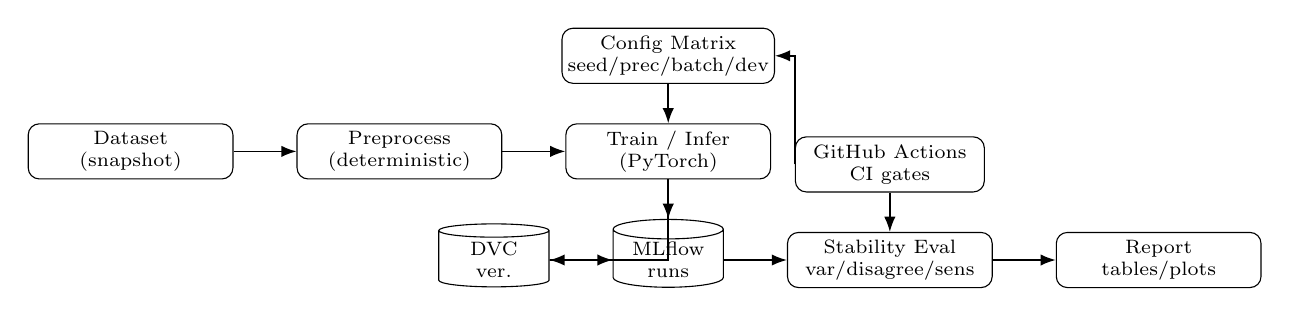
\begin{tikzpicture}[
    font=\scriptsize,
    node distance=5mm and 8mm,
    block/.style={draw, rounded corners, align=center, minimum width=26mm, minimum height=7mm, inner sep=2pt},
    smallblock/.style={draw, rounded corners, align=center, minimum width=24mm, minimum height=7mm, inner sep=2pt},
    datastore/.style={draw, cylinder, shape border rotate=90, aspect=0.25, align=center, minimum height=8mm, minimum width=14mm, inner sep=1pt},
    arrow/.style={-Latex, line width=0.55pt}
]

% ---------- Top row (compact) ----------
\node[block] (data) {Dataset\\(snapshot)};
\node[block, right=of data] (prep) {Preprocess\\(deterministic)};
\node[block, right=of prep] (train) {Train / Infer\\(PyTorch)};
\node[smallblock, above=of train] (cfg) {Config Matrix\\seed/prec/batch/dev};

% ---------- Bottom row ----------
\node[datastore, below=of train] (mlflow) {MLflow\\runs};
\node[datastore, left=of mlflow] (dvc) {DVC\\ver.};
\node[block, right=of mlflow] (eval) {Stability Eval\\var/disagree/sens};
\node[smallblock, above=of eval] (ci) {GitHub Actions\\CI gates};
\node[block, right=of eval] (report) {Report\\tables/plots};

% ---------- Edges (no crossings) ----------
\draw[arrow] (data) -- (prep);
\draw[arrow] (prep) -- (train);
\draw[arrow] (cfg) -- (train);

\draw[arrow] (train) -- (mlflow);
\draw[arrow] (train.south) |- (dvc.east);

\draw[arrow] (dvc) -- (mlflow);
\draw[arrow] (mlflow) -- (eval);
\draw[arrow] (ci) -- (eval);
\draw[arrow] (eval) -- (report);

% CI feedback loop to config (routed cleanly)
\draw[arrow] (ci.west) |- (cfg.east);

\end{tikzpicture}%
}
\caption{Compact pipeline for detecting numerical instability using an MLOps/DevOps toolchain.}
\label{fig:system_diagram}
\end{figure}




\section*{Evaluation Criteria}
Model performance will be evaluated using standard accuracy metrics to confirm functional correctness. Additional operational metrics will include prediction variance across runs, disagreement rates between model artifacts, sensitivity to small input perturbations, gradient norm behavior, and reproducibility gaps across identical configurations. All metrics will be logged and analyzed through MLflow, with datasets and artifacts versioned via Git/DVC and validated via CI automation.

\section*{Expected Outcomes}
The expected outcome is evidence that machine learning models can remain accurate while exhibiting numerically fragile behavior under realistic operational conditions. The project is expected to show that conventional validation practices may fail to detect these issues unless numerical robustness is explicitly monitored and enforced through CI gates.

\end{document}
